\part{系统功能}

在本节中,我将对YaDNS的主要功能特性进行介绍。

\begin{figure}
	\centering
	\subfloat[命令行帮助界面]{
		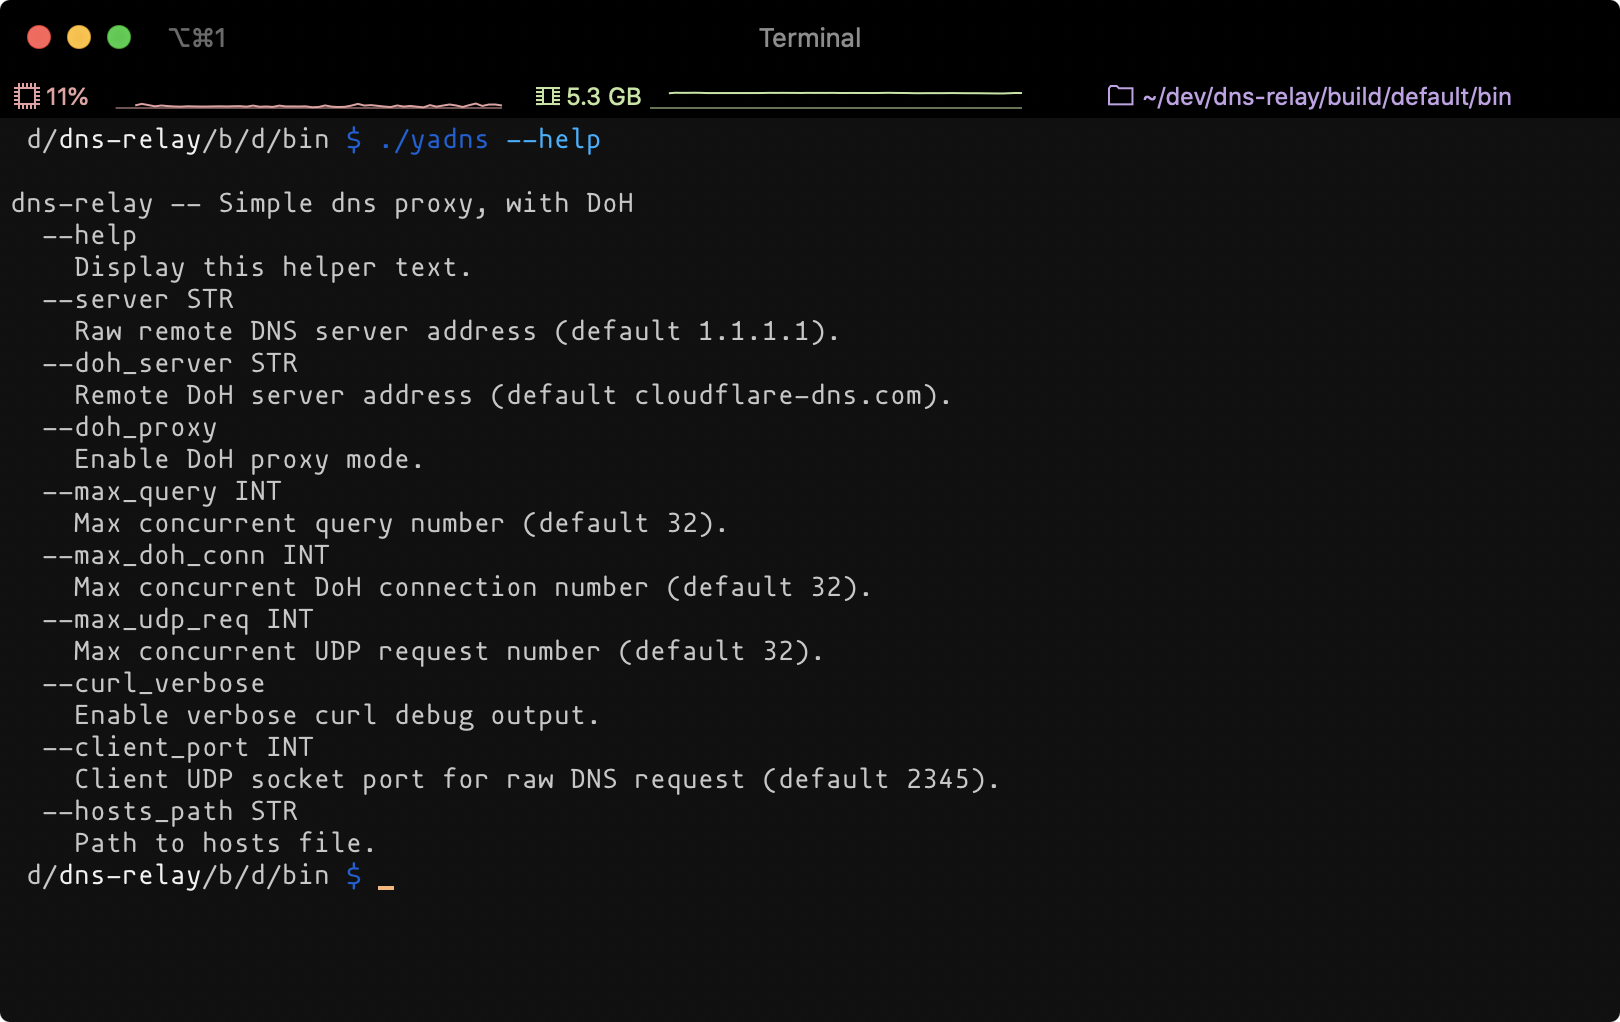
\includegraphics[width=0.43\textwidth]{figures/cli}
	}
	\enspace
	\subfloat[DoH运行界面]{
		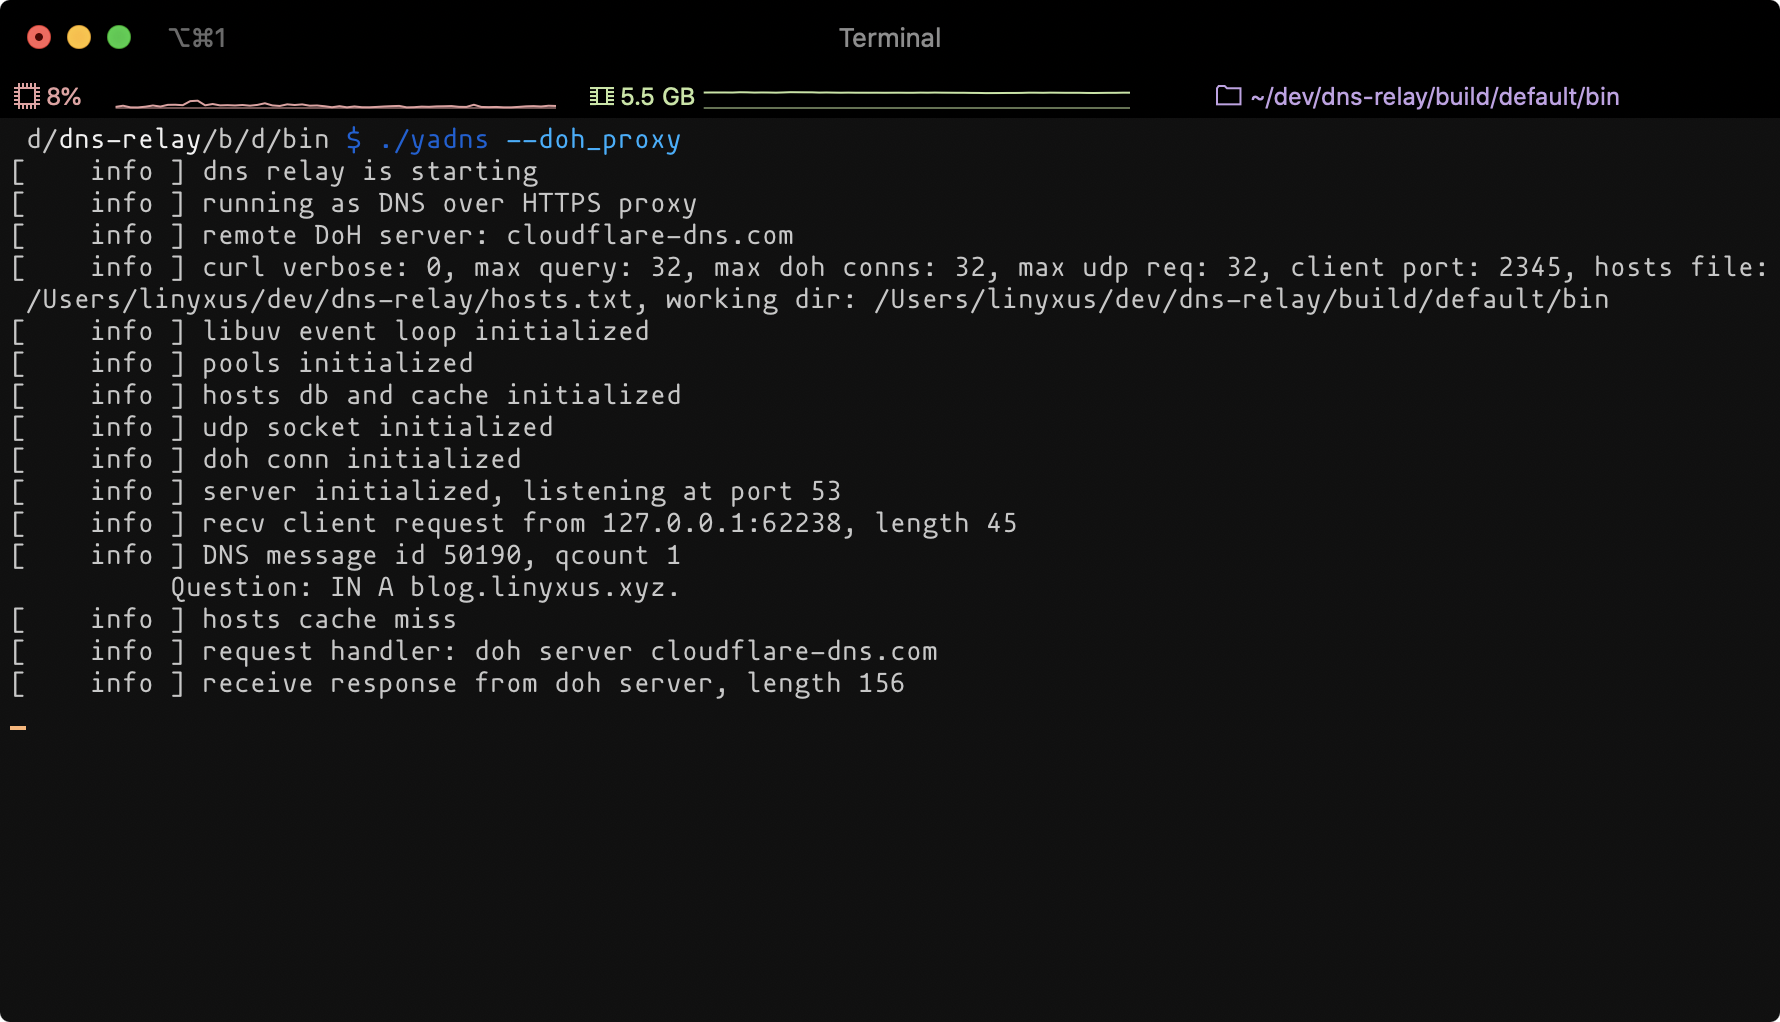
\includegraphics[width=0.47\textwidth]{figures/doh_proxy}
	}
	\label{fig:feature-showoff}
\end{figure}

\section{命令行用户界面}

YaDNS提供了丰富全面而友好的用户界面。提供了丰富的命令行选项,给出\lstinline{--help}标志则会打印出所有选项的帮助信息,也即
\begin{verbatim}
  ./yadns --help
\end{verbatim}

YaDNS在命令行界面中,提供了修改远程DNS服务器地址、修改远端DoH服务器接口、修改并行数等功能。在接下来会分别详细介绍。

\section{DNS over HTTPS}

DNS over HTTPS是一种基于HTTPS的新型DNS查询方式。传统的DNS查询方式很多都基于UDP进行明文传输,不进行加密也没有验证机制。这导致中间人可以很容易地窃听用户的DNS查询行为,泄露用户隐私。也能够篡改DNS报文内容以进行攻击,如DNS劫持。

HTTPS是增加了TLS \emph{(Transport Layer Security)}的HTTP请求。通过TLS规定的密码学方法,将HTTP报文内容加密,阻止中间人篡改、窃听客户端与服务器之间的HTTP流量。

DNS over HTTPS \emph{(DoH)} 将一次普通的DNS查询请求以HTTPS请求与响应的方式完成。DoH客户端将DNS报文包裹在HTTPS请求中发送给服务器,而服务器返回的HTTPS响应中包含了DNS查询结果。通过利用HTTPS的安全性,保证了原本明文传输的DNS请求不被窃听、篡改。保证了用户的隐私安全与网络安全。

YaDNS实现了DoH代理的功能。在本地运行YaDNS,并给出\lstinline{--doh_proxy}标志,并可以通过\lstinline{--doh_server}选项指定DoH服务器地址(默认为\lstinline{cloudflare-dns.com}),例如
\begin{verbatim}
  ./yadns --doh_proxy --doh_server cloudflare-dns.com
\end{verbatim}
则可以在本地启动一个DoH代理。将首选DNS服务器地址修改为\lstinline{127.0.0.1},则在访问互联网式产生的DNS查询,都将被YaDNS以DoH方式转发给远程服务器。通过这种方式,不安全的DNS流量被转化为了安全的DoH流量,在启用DoH Proxy之后,DNS污染、DNS劫持等威胁网络安全的行为,应当都不会发生了。

\section{并发连接池}

YaDNS实现了对请求的处理与转发的并发。当YaDNS接口收到了用户发来的请求之后,若没有命中本地加载的域名信息记录,需要转发到远端服务器,则会将请求存入查询池,并从请求池(对于UDP转发)或连接池(对于DoH转发)获取一个请求或连接处理器,负责向远端服务器发起请求。

请求的接收与发送都是异步的,利用\lstinline{libuv}\footnote{关于使用\lstinline{libuv}而非系统提供的轮询\emph{(poll)}接口来实现并发的原因与考虑,参见附录 \ref{sec:why-libuv}。}实现了基于事件循环的并发。可以通过命令行选项\lstinline{--max_query}, \lstinline{--max_doh_conn}, \lstinline{--max_udp_req}来规定查询池、请求池、连接池的大小,也就规定了最大的并发数量。

\section{多叉查找树与LRU缓存}

YaDNS支持加载本地的域名记录,当查询的域名在本地记录中时,YaDNS将直接返回DNS响应而不转发到远端服务器。

在查找本地记录时,YaDNS首先查找记录是否在LRU缓存中。LRU缓存采用LRU \emph{(Least Recently Used)} 换出策略,查找仅需常量时间;若没有命中缓存,则在多叉查找树中进行查找。LRU缓存与多叉查找树的效率在第 \ref{sec:time-space-complexity} 节中给出了详细的分析。

\section{基于 \lstinline{Trie} 树的响应缓存}

YaDNS支持对收到的远端服务器的响应中的 \textbf{A 类} 资源进行缓存。在YaDNS收到查询,发现查询没有命中本地记录时,将首先在响应缓存中进行查找,若查找到记录(且未过期),则直接将记录返回。在收到远端服务器返回的请求时,则会查看回答与权威节,若其中的记录为A类,则将域名-IP地址队存入 \lstinline{Trie} 树中。

缓存的资源记录的有效时间由报文中的TTL决定。对于过期域名记录的清理是惰性的,这意味着只有当一条过期的域名被查询到时,才会将其删除。在清除过期信息之后,会对 \lstinline{Trie} 树进行清理,删除无用节点。

